
%% bare_conf.tex
%% V1.4b
%% 2015/08/26
%% by Michael Shell
%% See:
%% http://www.michaelshell.org/
%% for current contact information.
%%
%% This is a skeleton file demonstrating the use of IEEEtran.cls
%% (requires IEEEtran.cls version 1.8b or later) with an IEEE
%% conference paper.
%%
%% Support sites:
%% http://www.michaelshell.org/tex/ieeetran/
%% http://www.ctan.org/pkg/ieeetran
%% and
%% http://www.ieee.org/

%%*************************************************************************
%% Legal Notice:
%% This code is offered as-is without any warranty either expressed or
%% implied; without even the implied warranty of MERCHANTABILITY or
%% FITNESS FOR A PARTICULAR PURPOSE! 
%% User assumes all risk.
%% In no event shall the IEEE or any contributor to this code be liable for
%% any damages or losses, including, but not limited to, incidental,
%% consequential, or any other damages, resulting from the use or misuse
%% of any information contained here.
%%
%% All comments are the opinions of their respective authors and are not
%% necessarily endorsed by the IEEE.
%%
%% This work is distributed under the LaTeX Project Public License (LPPL)
%% ( http://www.latex-project.org/ ) version 1.3, and may be freely used,
%% distributed and modified. A copy of the LPPL, version 1.3, is included
%% in the base LaTeX documentation of all distributions of LaTeX released
%% 2003/12/01 or later.
%% Retain all contribution notices and credits.
%% ** Modified files should be clearly indicated as such, including  **
%% ** renaming them and changing author support contact information. **
%%*************************************************************************


% *** Authors should verify (and, if needed, correct) their LaTeX system  ***
% *** with the testflow diagnostic prior to trusting their LaTeX platform ***
% *** with production work. The IEEE's font choices and paper sizes can   ***
% *** trigger bugs that do not appear when using other class files.       ***                          ***
% The testflow support page is at:
% http://www.michaelshell.org/tex/testflow/



\documentclass[conference]{IEEEtran}
% Some Computer Society conferences also require the compsoc mode option,
% but others use the standard conference format.
%
% If IEEEtran.cls has not been installed into the LaTeX system files,
% manually specify the path to it like:
% \documentclass[conference]{../sty/IEEEtran}





% Some very useful LaTeX packages include:
% (uncomment the ones you want to load)


% *** MISC UTILITY PACKAGES ***
%
%\usepackage{ifpdf}
% Heiko Oberdiek's ifpdf.sty is very useful if you need conditional
% compilation based on whether the output is pdf or dvi.
% usage:
% \ifpdf
%   % pdf code
% \else
%   % dvi code
% \fi
% The latest version of ifpdf.sty can be obtained from:
% http://www.ctan.org/pkg/ifpdf
% Also, note that IEEEtran.cls V1.7 and later provides a builtin
% \ifCLASSINFOpdf conditional that works the same way.
% When switching from latex to pdflatex and vice-versa, the compiler may
% have to be run twice to clear warning/error messages.






% *** CITATION PACKAGES ***
%
%\usepackage{cite}
% cite.sty was written by Donald Arseneau
% V1.6 and later of IEEEtran pre-defines the format of the cite.sty package
% \cite{} output to follow that of the IEEE. Loading the cite package will
% result in citation numbers being automatically sorted and properly
% "compressed/ranged". e.g., [1], [9], [2], [7], [5], [6] without using
% cite.sty will become [1], [2], [5]--[7], [9] using cite.sty. cite.sty's
% \cite will automatically add leading space, if needed. Use cite.sty's
% noadjust option (cite.sty V3.8 and later) if you want to turn this off
% such as if a citation ever needs to be enclosed in parenthesis.
% cite.sty is already installed on most LaTeX systems. Be sure and use
% version 5.0 (2009-03-20) and later if using hyperref.sty.
% The latest version can be obtained at:
% http://www.ctan.org/pkg/cite
% The documentation is contained in the cite.sty file itself.






% *** GRAPHICS RELATED PACKAGES ***
%
\ifCLASSINFOpdf
\usepackage[pdftex]{graphicx}
\usepackage{amsmath}
  % \usepackage[pdftex]{graphicx}
  % declare the path(s) where your graphic files are
  % \graphicspath{{../pdf/}{../jpeg/}}
  % and their extensions so you won't have to specify these with
  % every instance of \includegraphics
  % \DeclareGraphicsExtensions{.pdf,.jpeg,.png}
\else
  % or other class option (dvipsone, dvipdf, if not using dvips). graphicx
  % will default to the driver specified in the system graphics.cfg if no
  % driver is specified.
  % \usepackage[dvips]{graphicx}
  % declare the path(s) where your graphic files are
  % \graphicspath{{../eps/}}
  % and their extensions so you won't have to specify these with
  % every instance of \includegraphics
  % \DeclareGraphicsExtensions{.eps}
\fi
% graphicx was written by David Carlisle and Sebastian Rahtz. It is
% required if you want graphics, photos, etc. graphicx.sty is already
% installed on most LaTeX systems. The latest version and documentation
% can be obtained at: 
% http://www.ctan.org/pkg/graphicx
% Another good source of documentation is "Using Imported Graphics in
% LaTeX2e" by Keith Reckdahl which can be found at:
% http://www.ctan.org/pkg/epslatex
%
% latex, and pdflatex in dvi mode, support graphics in encapsulated
% postscript (.eps) format. pdflatex in pdf mode supports graphics
% in .pdf, .jpeg, .png and .mps (metapost) formats. Users should ensure
% that all non-photo figures use a vector format (.eps, .pdf, .mps) and
% not a bitmapped formats (.jpeg, .png). The IEEE frowns on bitmapped formats
% which can result in "jaggedy"/blurry rendering of lines and letters as
% well as large increases in file sizes.
%
% You can find documentation about the pdfTeX application at:
% http://www.tug.org/applications/pdftex





% *** MATH PACKAGES ***
%
%\usepackage{amsmath}
% A popular package from the American Mathematical Society that provides
% many useful and powerful commands for dealing with mathematics.
%
% Note that the amsmath package sets \interdisplaylinepenalty to 10000
% thus preventing page breaks from occurring within multiline equations. Use:
%\interdisplaylinepenalty=2500
% after loading amsmath to restore such page breaks as IEEEtran.cls normally
% does. amsmath.sty is already installed on most LaTeX systems. The latest
% version and documentation can be obtained at:
% http://www.ctan.org/pkg/amsmath





% *** SPECIALIZED LIST PACKAGES ***
%
%\usepackage{algorithmic}
% algorithmic.sty was written by Peter Williams and Rogerio Brito.
% This package provides an algorithmic environment fo describing algorithms.
% You can use the algorithmic environment in-text or within a figure
% environment to provide for a floating algorithm. Do NOT use the algorithm
% floating environment provided by algorithm.sty (by the same authors) or
% algorithm2e.sty (by Christophe Fiorio) as the IEEE does not use dedicated
% algorithm float types and packages that provide these will not provide
% correct IEEE style captions. The latest version and documentation of
% algorithmic.sty can be obtained at:
% http://www.ctan.org/pkg/algorithms
% Also of interest may be the (relatively newer and more customizable)
% algorithmicx.sty package by Szasz Janos:
% http://www.ctan.org/pkg/algorithmicx




% *** ALIGNMENT PACKAGES ***
%
%\usepackage{array}
% Frank Mittelbach's and David Carlisle's array.sty patches and improves
% the standard LaTeX2e array and tabular environments to provide better
% appearance and additional user controls. As the default LaTeX2e table
% generation code is lacking to the point of almost being broken with
% respect to the quality of the end results, all users are strongly
% advised to use an enhanced (at the very least that provided by array.sty)
% set of table tools. array.sty is already installed on most systems. The
% latest version and documentation can be obtained at:
% http://www.ctan.org/pkg/array


% IEEEtran contains the IEEEeqnarray family of commands that can be used to
% generate multiline equations as well as matrices, tables, etc., of high
% quality.




% *** SUBFIGURE PACKAGES ***
%\ifCLASSOPTIONcompsoc
%  \usepackage[caption=false,font=normalsize,labelfont=sf,textfont=sf]{subfig}
%\else
%  \usepackage[caption=false,font=footnotesize]{subfig}
%\fi
% subfig.sty, written by Steven Douglas Cochran, is the modern replacement
% for subfigure.sty, the latter of which is no longer maintained and is
% incompatible with some LaTeX packages including fixltx2e. However,
% subfig.sty requires and automatically loads Axel Sommerfeldt's caption.sty
% which will override IEEEtran.cls' handling of captions and this will result
% in non-IEEE style figure/table captions. To prevent this problem, be sure
% and invoke subfig.sty's "caption=false" package option (available since
% subfig.sty version 1.3, 2005/06/28) as this is will preserve IEEEtran.cls
% handling of captions.
% Note that the Computer Society format requires a larger sans serif font
% than the serif footnote size font used in traditional IEEE formatting
% and thus the need to invoke different subfig.sty package options depending
% on whether compsoc mode has been enabled.
%
% The latest version and documentation of subfig.sty can be obtained at:
% http://www.ctan.org/pkg/subfig




% *** FLOAT PACKAGES ***
%
%\usepackage{fixltx2e}
% fixltx2e, the successor to the earlier fix2col.sty, was written by
% Frank Mittelbach and David Carlisle. This package corrects a few problems
% in the LaTeX2e kernel, the most notable of which is that in current
% LaTeX2e releases, the ordering of single and double column floats is not
% guaranteed to be preserved. Thus, an unpatched LaTeX2e can allow a
% single column figure to be placed prior to an earlier double column
% figure.
% Be aware that LaTeX2e kernels dated 2015 and later have fixltx2e.sty's
% corrections already built into the system in which case a warning will
% be issued if an attempt is made to load fixltx2e.sty as it is no longer
% needed.
% The latest version and documentation can be found at:
% http://www.ctan.org/pkg/fixltx2e


%\usepackage{stfloats}
% stfloats.sty was written by Sigitas Tolusis. This package gives LaTeX2e
% the ability to do double column floats at the bottom of the page as well
% as the top. (e.g., "\begin{figure*}[!b]" is not normally possible in
% LaTeX2e). It also provides a command:
%\fnbelowfloat
% to enable the placement of footnotes below bottom floats (the standard
% LaTeX2e kernel puts them above bottom floats). This is an invasive package
% which rewrites many portions of the LaTeX2e float routines. It may not work
% with other packages that modify the LaTeX2e float routines. The latest
% version and documentation can be obtained at:
% http://www.ctan.org/pkg/stfloats
% Do not use the stfloats baselinefloat ability as the IEEE does not allow
% \baselineskip to stretch. Authors submitting work to the IEEE should note
% that the IEEE rarely uses double column equations and that authors should try
% to avoid such use. Do not be tempted to use the cuted.sty or midfloat.sty
% packages (also by Sigitas Tolusis) as the IEEE does not format its papers in
% such ways.
% Do not attempt to use stfloats with fixltx2e as they are incompatible.
% Instead, use Morten Hogholm'a dblfloatfix which combines the features
% of both fixltx2e and stfloats:
%
% \usepackage{dblfloatfix}
% The latest version can be found at:
% http://www.ctan.org/pkg/dblfloatfix




% *** PDF, URL AND HYPERLINK PACKAGES ***
%
%\usepackage{url}
% url.sty was written by Donald Arseneau. It provides better support for
% handling and breaking URLs. url.sty is already installed on most LaTeX
% systems. The latest version and documentation can be obtained at:
% http://www.ctan.org/pkg/url
% Basically, \url{my_url_here}.




% *** Do not adjust lengths that control margins, column widths, etc. ***
% *** Do not use packages that alter fonts (such as pslatex).         ***
% There should be no need to do such things with IEEEtran.cls V1.6 and later.
% (Unless specifically asked to do so by the journal or conference you plan
% to submit to, of course. )


% correct bad hyphenation here
\hyphenation{op-tical net-works semi-conduc-tor}


\begin{document}
%
% paper title
% Titles are generally capitalized except for words such as a, an, and, as,
% at, but, by, for, in, nor, of, on, or, the, to and up, which are usually
% not capitalized unless they are the first or last word of the title.
% Linebreaks \\ can be used within to get better formatting as desired.
% Do not put math or special symbols in the title.
\title{Distributed Vision-Based Target Tracking Control Using Multiple Mobile Robots}


% author names and affiliations
% use a multiple column layout for up to three different
% affiliations
\author
{\IEEEauthorblockN{Dr Jing Wang}
\IEEEauthorblockA{School of Electrical and\\Computer Engineering\\
Bradley University\\
Peoria, IL 61606\\
jingwang@fsmail.bradley.edu}
\and
\IEEEauthorblockN{Dr In Soo Ahn}
\IEEEauthorblockA{School of Electrical and\\Computer Engineering\\
Bradley University\\
Peoria, IL 61606\\
isa@fsmail.bradley.edu }
\\
\IEEEauthorblockN{Anthony Le}
\IEEEauthorblockA{School of Electrical and\\Computer Engineering\\
Bradley University\\
Peoria, IL 61606\\
ale@mail.bradley.edu  }
\and
\IEEEauthorblockN{Ryan Clue}
\IEEEauthorblockA{School of Electrical and\\Computer Engineering\\
Bradley University\\
Peoria, IL 61606\\
rclue@mail.bradley.edu }}

% conference papers do not typically use \thanks and this command
% is locked out in conference mode. If really needed, such as for
% the acknowledgment of grants, issue a \IEEEoverridecommandlockouts
% after \documentclass

% for over three affiliations, or if they all won't fit within the width
% of the page, use this alternative format:
% 
%\author{\IEEEauthorblockN{Michael Shell\IEEEauthorrefmark{1},
%Homer Simpson\IEEEauthorrefmark{2},
%James Kirk\IEEEauthorrefmark{3}, 
%Montgomery Scott\IEEEauthorrefmark{3} and
%Eldon Tyrell\IEEEauthorrefmark{4}}
%\IEEEauthorblockA{\IEEEauthorrefmark{1}School of Electrical and Computer Engineering\\
%Georgia Institute of Technology,
%Atlanta, Georgia 30332--0250\\ Email: see http://www.michaelshell.org/contact.html}
%\IEEEauthorblockA{\IEEEauthorrefmark{2}Twentieth Century Fox, Springfield, USA\\
%Email: homer@thesimpsons.com}
%\IEEEauthorblockA{\IEEEauthorrefmark{3}Starfleet Academy, San Francisco, California 96678-2391\\
%Telephone: (800) 555--1212, Fax: (888) 555--1212}
%\IEEEauthorblockA{\IEEEauthorrefmark{4}Tyrell Inc., 123 Replicant Street, Los Angeles, California 90210--4321}}




% use for special paper notices
%\IEEEspecialpapernotice{(Invited Paper)}




% make the title area
\maketitle

% As a general rule, do not put math, special symbols or citations
% in the abstract
\begin{abstract}
In this project, a distributed vision-based control system is designed for mobile robots to address the target tracking problem while maintaining the specified formation among robots. The system mainly consists of two modules. One is for target identification and the other is for target tracking control. In the target identification module, the robot is controlled to pivot around its center and perform a survey of the environment using its on-board vision sensor. In the target tracking control module, a leader-follower control strategy is adopted to solve the target tracking and formation control problem of multiple robots. The proposed distributed vision-based control is experimentally tested using three QBot2s from Quanser, Inc. 
\end{abstract}

% no keywords




% For peer review papers, you can put extra information on the cover
% page as needed:
% \ifCLASSOPTIONpeerreview
% \begin{center} \bfseries EDICS Category: 3-BBND \end{center}
% \fi
%
% For peerreview papers, this IEEEtran command inserts a page break and
% creates the second title. It will be ignored for other modes.
\IEEEpeerreviewmaketitle



\section{Introduction}

\subsection{Motivation}

Distributed control of multiple unmanned autonomous robots (UARs) has been the subject of intensive research in recent years due to the potential applications in search and rescue missions, surveillance and reconnaissance, environmental sensing and monitoring, intelligent transportation and threat isolation/evasion, and obstacle evasion [1]. There are many practical commercial, civil and military applications that may benefit from advancements in UAR control strategies and algorithms from this area of research. 

\subsection{Related Work}
Methods for successfully coordinating multiple robots to autonomously encircle a target point have been put forth by several research papers.  These distributed controls assume communication the robots to communicate their kinematic state variables between one another, and consequently researchers have designed their algorithms in ways that minimize the number of communication channels required between robots.  However, there has not been nearly as much research done that attempt to implement coordinated encirclement that rely entirely on each individual robot’s vision sensors.

A review of prior work at Bradley and research literature was conducted by our team during the conception phase of the project.  This included a review of e prior Class of 2016 Senior Project, Cooperative Control of Heterogeneous Mobile Robots Network [cite ref 1?]. The 2016 research and capstone project experience using the QBot2 robots was leveraged in our project. The 2016 project tested cooperative control using the QBot2 platform including the Qbot2 Camera and the Kinect RGBD camera for localization.  Wifi communication was used to exchange position information among robots. Consensus and formation stabilization problems were studied. 

Our project also researched and references another work, highly relevant to our 2017 project objectives. Decentralized multi-robot encirclement of a 3D target with guaranteed collision avoidance for object tracking and encirclement by Franchi, Stegagno, and Oriolo, [cite ref 2]. Their work on 3-D (and 2-D) and distributed collaborative control is extensive and leverages research going back to 2001.   Their findings delivers a control framework for achieving encirclement of a target moving in a 3D space using multiple robots, image-only sensing, and requiring local communication between exactly two other members of the encircling group of robots. 

An additional consideration, for a vision-only sensing strategy was image processing techniques and algorithms.  We relied on Peter Corke’s book “Robotics, Vision and Control” as well as his Matlab toolbox for much of our image processing.  The academic tutorials packaged with the Qbot2 were also valuable resources.  It is worth mentioning that systems in the literature utilizing visual-only sensing generally assumed 360-degree robot sensing (e.g. fisheye camera). Ref 1 Research (extracts below) utilized a 240deg field of view sensor and a laser range finder for identification and locating targets to support inputs to their control strategies.  Because the Qbot2 cameras have less than a 90-degree field-of-view, our design would have to incorporate additional logic to locate targets outside the robot’s visual range.

\section{Problem Formulation}


\subsection{Kinematic Model of Mobile Robots}

Depending on whether the robot is following a target or leader robots, two separate control modules are used. Both modules use a Cartesian coordinate system and follow a target point, which is obtained by transforming the current or previous result of the image processing module with respect to the robot’s current position.

\subsection{Vision-based control}
The purpose of the vision-based control is to provide a target point to the kinematic control, which it accomplishes by processing the Qbot2’s color images and depth images. This control should also provide additional information as to whether the target point it provides should be considered valid or not.


\subsection{Project Objectives, Goals, and Approach}
The goal of our project is to design distributed vision-based control algorithms for mobile robots and to implement and validate the proposed algorithms. The primary project tasks (research, concept definition, design, and demonstration) tasks included:

\begin{itemize}
\item	Design a target identification (detect and locate) module based on RGB image features obtained from a vision sensor
\item	Design a target tracking algorithm based on robot model linearization
\item	Design a leader-follower formation control algorithm based on depth and image features provided from the target identification module 
\item	Design a state machine to coordinate target identification module and target control module and communications between Robots
\item	Integrate and validate the proposed distributed controls through experimentation in a controlled lab environment
\end{itemize}


\subsection{Project Assumptions}
The Lab environment, limitations of the research and practical limitations (and availability) of fully operational equipment are also considered.  

\begin{itemize}
\item	The lab environment will be a well-lit, indoor area
\item	The target will remain on the same level plane as the robots (2D motion tracking).  
\item	The target will not move faster than the Qbot2s maximum velocity (0.7 m/s).  
\item	The target will be a solid colored, basketball-sized sphere.  
\item	The environment will be reasonably free of similarly colored objects.  
\item	As stated above the multiple robots must use same control strategy.

\end{itemize}
\section{Design of Distributed Vision-based Control}


\subsection{Design approach}

The basic “system” is comprised of the QBot2 Mobile Robot and QUARK Control Software on a host computer.  The full “system” is comprised of multiple QBot2s collaboratively tracking a single target with the Quark Control Software Computer.  Note: An assumption is that the Quark Control Software on the host computer could be ported entirely to the robots, given sufficient processing and communications, to attain higher autonomy and actual decentralization of the system.  The target in the experiment is a round ball that is detected, located, and tracked by the multiple QBot2s.    
Subsystems for the basic system, a single QBot2, include: the Qbot2 mechanical/motors/control subsystem, the sensing/image processing subsystem, and the communications/processing subsystems (on the Qbot2 and the Host computer). 

\subsection{QBot2 Mobile Robot and QUARC Platform}

The QBot2 utilizes QUARC’s HIL software suite to allow users to design their program using Matlab and Simulink.  The Simulink model and Matlab code are translated to C++ code by the QUARC software and compiled automatically on the Qbot2’s computer.

\subsubsection{Hardware}

The QBot2 comes equipped with a differential drive robot base which has a maximum speed of 0.7m/s. A v.1 Kinect-for-Xbox mounted on the robot base provides both color and distance vision information.  The RGB image that has a default resolution of 640 $\times$ 480 pixels and a 57° $\times$ 43° field of view.  The depth image has a resolution of 640 $\times$ 480 pixels, approximately 52.5° $\times$ 41° field of view, and measures distances from 0.5m to 6.0m. It is worth noting that the accuracy of the depth map depends on the detail of the grid projected by the IR emitter, the actual accuracy of the depth image is significantly lower than a resolution of 640x480 implies.   QBots use IEEE 802.11 b/g/n protocol for communication between the computer and QBot2. TCP/IP protocol is utilized, with each QBot2 using a statically assigned IP address. 
\begin{figure}[htbp] %  figure placement: here, top, bottom, or page
     \centering
     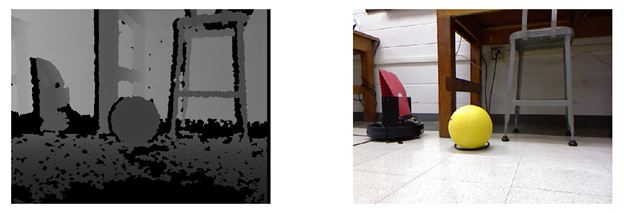
\includegraphics[width=3in]{1.png} 
     \caption{Side-By-Side of Color and Depth Images}
     \label{fig:1}
  \end{figure}     


\begin{figure}[htbp] %  figure placement: here, top, bottom, or page
     \centering
     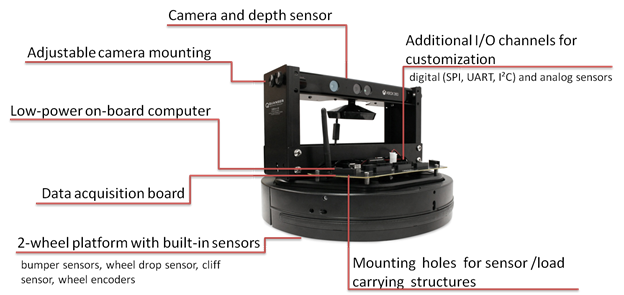
\includegraphics[width=3in]{2.png} 
     \caption{QBot2 Mobile Robot}
     \label{fig:2}
  \end{figure}     


\subsubsection{Software}
To connect to the QBOT2 A host-target real-time control system [2] is utilized.   As shown in Figure 3-2, the target QBOT2 computer is connected wirelessly with the host computer on which the SIMULINK model is running. The control algorithms are developed in MATLAB/SIMULINK with QUARC on the host computer. The control models are cross-compiled and downloaded to the target computer in real time. 


\begin{figure}[htbp]
\begin{center}
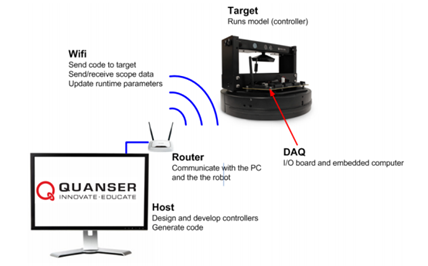
\includegraphics[width=3in]{3}
\caption{Host Computer / Wi-Fi Router to Qbot Communications Connectivity} \label{fig:3}
\end{center}
\end{figure}

\subsection{Target Identification}
\subsubsection{Interface and inputs to Target Control}
The result of the vision control system is a target location given in 2D Cartesian coordinates. The origin of this coordinate plane is at the Qbot2’s camera position, the positive X axis extends in same the direction the Kinect is facing and the positive Y axis extends to the left (or “port” side) of the Kinect.  The motion control module will then transform this point according to its current kinematic state.   This is target point is the basic interface between the target identification module and the motion control.

Based on the 2016 Senior Project, and research of alternatives, we chose to use the color image for object/target recognition and the depth image for determining distance to the target. Our choice was driven primarily by practical QBot2 processing limitations and timing restrictions prohibiting potentially more robust methods of object detection.

\subsubsection{Acquire Y Component of Target Location from Color Imagel}
We perform all object recognition on the color image.  Consequently, color image processing is the primary bottleneck in system performance.  We initially selected color thresholding with blob detection because it is the easiest image processing method to implement.  Although we did pursue alternative methods of image processing, these implementations were unable to meet our performance requirements due to limitations of the Qbot2 hardware.  Therefore, color thresholding with blob detection was selected because it had a significantly lower performance requirement while also producing adequate results. 

The first stage of image processing, color thresholding, highlights all elements of the image that correspond to our target’s color.  During this stage, pixels with RGB values that fall within a pre-determined range are replaced by ‘1’ in the binary output image, while all other values are replaced by ‘0’.  
\begin{figure}[htbp]
\begin{center}
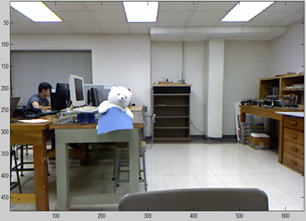
\includegraphics[width=3in]{4}
\caption{Before Processing - Color Thresholding and Blob Detection} \label{fig:4}
\end{center}
\end{figure}

\begin{figure}[htbp]
\begin{center}
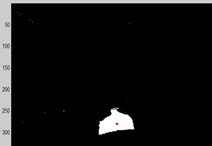
\includegraphics[width=3in]{5}
\caption{After Processing - Color Thresholding and Blob Detection} \label{fig:5}
\end{center}
\end{figure}
Blob detection is applied to the binary output image from color thresholding.  The goal is to identify the largest grouping of neighboring, non-zero values.  Then, for each group (or “blob”) of neighboring pixels, we calculate its centroid by finding the mean index of all pixels contained in that blob.  This means that the accuracy of the blob corresponding to our target object is unaffected by “noise” from similar colors appearing elsewhere in the image.  It should be noted that the accuracy of this method is therefore entirely dependent on the color thresholding result.  



The blob detection outputs a list of centroids and corresponding blob sizes.  If the blob size of the largest blob is greater than some pre-determined threshold value, our system will use that centroid for the target’s coordinates on the RGB image plane. 


\subsubsection{Acquire X Component of Target Location from Depth Image}
The target’s location on the depth map can be estimated by translating points from the color image plane to the depth image plane.  We calculated this using the ratio between the two images’ field-of-view and the estimated angle from the RGB image.

\begin{figure}[htbp]
\begin{center}
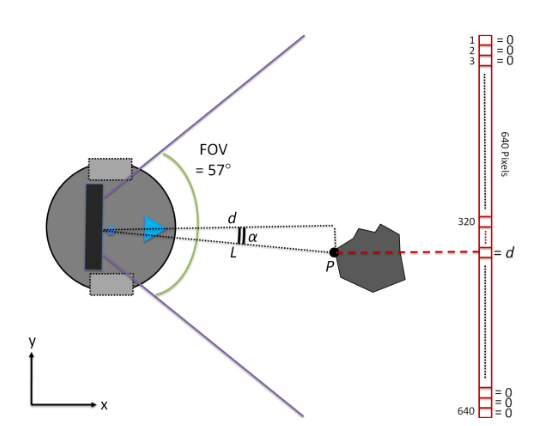
\includegraphics[width=3in]{6}
\caption{Target Localization - Finding Distance} \label{fig:6}
\end{center}
\end{figure}

\begin{equation}
∝_T=(L_{color}/2-X_{color} )(¬(FOV_{color}-x)/L_{color} )
\end{equation}

\begin{figure}[htbp]
\begin{center}
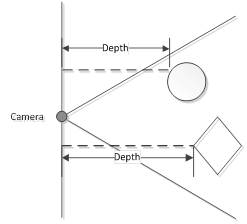
\includegraphics[width=3in]{7}
\caption{Target Localization - Determining x,y coordinates} \label{fig:7}
\end{center}
\end{figure}

\begin{equation}
\begin{aligned}
〖XY〗_{depth}= & (〖FOV〗_{color}/L_{color} ) (L_{depth}/〖FOV〗_{depth} )  \\  & *〖∙XY〗_{color}+offset
\end{aligned}
\end{equation}
\begin{equation}
X_T=〖Image〗_{depth} (X_{depth},Y_{depth})
\end{equation}
\begin{equation}
Y_T=X_T∙tan⁡(∝_T)
\end{equation}
\subsection{Motion Control}
\subsubsection{Encirclement}
The target control module relies on received target coordinates from the image processing module and the robot’s  x,y, and theta. These are inputs which allow for formulation of encirclement.  From the robot’s x,y, and theta values, we transform these values to the appropriate kinematic model for the QBot2. From this kinematic model, we transform the cartesian local coordinate system to a cylindrical coordinate system. The length between the two wheels of the QBot is 0.0235 meters. We use the stardard kinematic model,
\begin{equation}
\dot{x}=V_c*cos⁡(\theta)
\end{equation}
\begin{equation}
\dot{y} =V_c*sin⁡(\theta)
\end{equation}
\begin{equation}
\dot\theta=\omega_c
\end{equation}
to find the forward point of the robot,
\begin{equation}
	P_x=x+0.0235*cos⁡(\theta)
\end{equation}
\begin{equation}
	P_y=y+0.0235*sin⁡(\theta)
\end{equation}

\begin{figure}[htbp] %  figure placement: here, top, bottom, or page
     \centering
     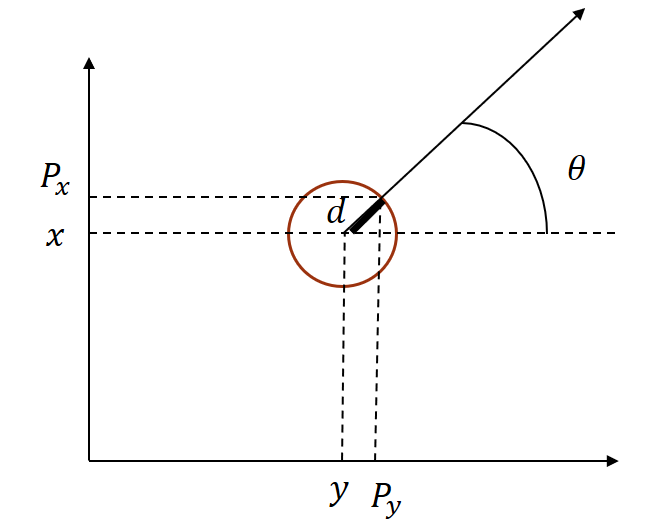
\includegraphics[width=3in]{7b.png} 
     \caption{$P_x$ and $P_y$ Conversion}
     \label{fig:7b}
  \end{figure}     

Following, we want to define $p_i$,
\begin{equation}
	p_i= (\rho_i , \phi_i)
\end{equation}
	
and convert these values by,
\begin{equation}
	\rho(P)= \sqrt{(P_{xd}^2+P_{yd}^2 ) }
\end{equation}
	
\begin{equation}
	\phi(p)= tan^{-1} ⁡(P_{yd},P_{xd})
\end{equation}
	

where P is the pose of the model.

$\dot{\rho}$ and $\dot{\phi}$ are the forward velocity and angular velocity computed by:
----
\begin{equation}
	\dot{\rho}=k_r*(\rho_s- \rho_d)
\end{equation}
		
\begin{equation}
	\dot{\phi}=\omega_d
\end{equation}
	

where $k_r$  is the porportional gain and $\rho_s$ is the size of the encirclement radius. $\rho_d$ is the approximate distance from the robot to the target given from the inverse kinematics and image processing modules.

We then use the Jacobian matrix of the difference between the target and robot where $P_x$ and $P_y$ is the X and Y coordinates of the robot and $P_{xt}$ and $P_{yt}$ is the X and Y coordinates of the target in relation to the robot’s coordinate frame. The difference of the robots X and Y locations can be reduced to $P_{xd}$ and $P_{yd}$. and the following Jacobian  matrix can be computed
\begin{equation}
	J_i =
\begin{bmatrix}
    P_{xd}/\sqrt{(P_{xd}^2+P_{yd}^2 )}      &   P_{yd}/\sqrt{(P_{xd}^2+P_{yd}^2 )}  \\
   -P_{yd}/(P_{xd}^2+P_{yd}^2 )      &  P_{xd}/(P_{xd}^2+P_{yd}^2)   
    
\end{bmatrix}
\end{equation}


	


From the Jacobian, the following input velocities Ux and Uy can be computed
\begin{equation}
		\begin{bmatrix}
		U_x\\U_y 
		\end{bmatrix}
		=J_i^{-1}*\begin{bmatrix}\dot\rho \\ \dot\phi ̇\end{bmatrix}
\end{equation}
	
For the velocity inputs, $U_x$ and $U_y$ , they are transformed using the inverse kinematic equations
\begin{equation}
			p^{-1}= \begin{bmatrix}cos⁡(\theta) & -0.0235*sin⁡(\theta) \\ sin⁡(\theta) & 0.0235*cos⁡(\theta) \end{bmatrix}^{-1}
\end{equation}
	
to find $V_c$ and $\omega_c$,
\begin{equation}
\begin{bmatrix} V_c \\ \omega_c \end{bmatrix}=p^{-1}*\begin{bmatrix}U_x \\ U_y\end{bmatrix}
\end{equation}	

Once $V_c$ and $W_c$ are found, using
\begin{equation}
V_r=V_c+1/2* .0235*2*\omega_c
\end{equation}
\begin{equation}
	V_L=V_c-1/2* .0235*2*\omega_c
\end{equation}
	

	
we can find velocities of the right and left wheels, $V_r$ and $V_L$.

Right and left wheel velocities are then sent to the HIL Write block which sends data to the 2000 and 2001 ports of the QBot2 for the left and right wheels, respectively.
The QBot2 stores wheel encoder data to allow calculation of actual right and left wheel velocities. This data is taken from the HIL Read block. For each wheel encoder ticks, we can determine the velocity of each wheel. The robot’s x,y, and $\theta$ values are then updated and sent back into the control module using $V_c$ and $\theta$ where,
\begin{equation}
V_c=0.5*(V_L+V_r)
\end{equation}
\begin{equation}
\theta=1/0.235*(V_r-V_L)
\end{equation}
	

	


From $V_c$ and $\omega_c$, we can determine the robot’s X, Y, and $\theta$ values by calculating the integrals for
\begin{equation}
\dot{x} =cos⁡(\theta)*V_c
\end{equation}
\begin{equation}
\dot{y}=sin⁡(\theta)*V_c
\end{equation}
\begin{equation}
	\dot\theta= \omega	
\end{equation}

	

		

\subsubsection{Leader-Follower}
Leader-follower control module is used for distributed multi-robot coordination. The leader-follower control module does not take into account inverse kinematics. And, the image processing is used to localize the leader robot coordinates ($x_r$  , $y_r$) in the vision sensor range. Given the radial distance of the target, $V_c$ and $\omega_c$ are calculated. A follow distance of 0.5 meters and gains  Kw = 0.5 and Kv = 0.2 were defined as per limitations for the QBot.
To determine $V_c$ and $\omega_c$,
\begin{equation}
	V_c=K_v*\sqrt{x_t^2+y_t^2 }-0.5
\end{equation}

\begin{equation}
	\omega_c=-K_w*tan^{-1}⁡(x_t,y_t)
\end{equation}


where $x_t$ and $y_t$ are the positions of the target in relation to the robot’s local coordinate frame.
One should note the limits for angular and forward velocity are set to .2 m/s.



\subsection{Event-based System Control}
\subsubsection{Implementation}
The Simulink model is configured using the HIL block from the QUARC toolbox.  This enables users to more easily run their simulations in a virtual environment as well as on actual hardware.  The project must also be configured to communicate with a specific IP address, which can be done through the QUARC add-on options menu in Simulink.  It is also important to set the sample time configure the “Solver” pane of the Simulink model configuration.  It is important to select the “ode1” and “fixed-step” options.  Additionally, when performing operations on images or large arrays of data, it is recommended that users select a sample frequency no greater than 15Hz.  Our experiments used a 10Hz sample frequency.
\subsubsection{Tasks Coordination}
Our system would need to switch between two modes of operation depending on whether or not the target was in view.   Stateflow was used to control the varying states in our model. Models for both target encirclement and leader-follower used similar simulink and stateflow models with differences only in controls and how often a search was made. In both models, search mode is done by toggling between image processing and rotating. Once the desired accuracy is obtained from blob detection, the state switched to the control module.  The target encirclement model only searches for target every set time-interaction whereas leader-follower will search for a target every other time-step. 
To view the entire Stateflow and its subsystem, see figure~\ref{fig:a8} to \ref{fig:a10} on page~\pageref{fig:a8} to \pageref{fig:a10}.

\begin{figure}[htbp]
\begin{center}
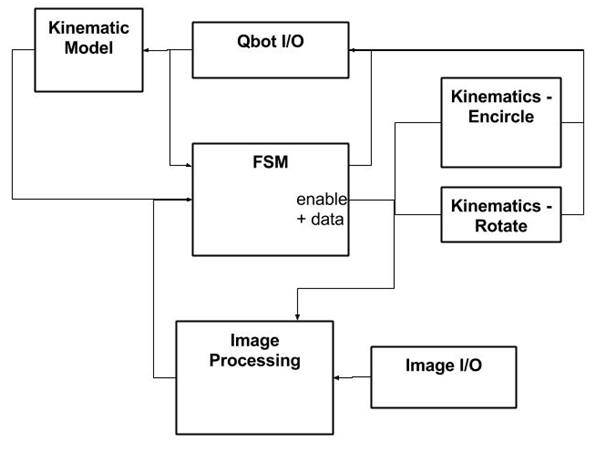
\includegraphics[width=3in]{8}
\caption{Abstracted View of Simulink Diagram} \label{fig:8}
\end{center}
\end{figure}

\subsubsection{Target Encirclement - Finite State Machine}
In the stateflow for target encirclement control, various enable switches allow triggering of different modules. The system starts off with all enable switches off. While entering target acquisition mode, image processing module is enabled and determines if an image centroid can be made. If no centroid is found, the QBot2 will rotate 15 degrees on its axis and wait for the cameras to update. If a centroid can be made, it checks whether the pixel size of the image is greater than a certain value. In our case, a yellow ball or box is used. If 30 pixels are connected, the robot will continue into the encirclement module. Data from the image processing, such as the robot’s x, y, and theta, is also sent to the encirclement module. From this module, the target location is stored and encirclement is based on this value. After 120 seconds, the encirclement ceases and target acquisition mode begins again. 

\begin{figure}[htbp]
\begin{center}
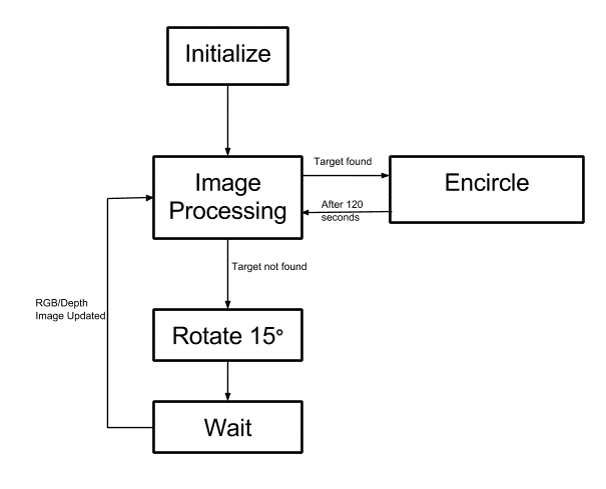
\includegraphics[width=3in]{9b}
\caption{Event-based System Control: Encirclement Control} \label{fig:9b}
\end{center}
\end{figure}

\subsubsection{Leader-Follower - Finite State Machine}

Leader-follower control is similar to target encirclement control. However, instead of returning to Target Acquisition mode, the target will continue to follow any centroid even if the pixel count is less than 30. The process is done by continually switching from image processing and the leader-follower control module. If no centroid is found, the target will return into Target Acquisition mode.


\begin{figure}[htbp] 
\begin{center}
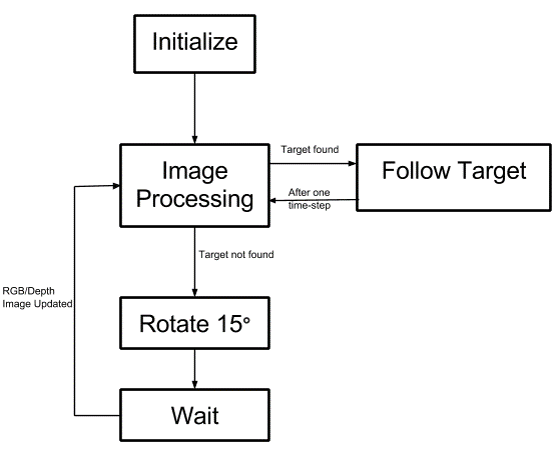
\includegraphics[width=3in]{10b}
\caption{Event-based System Control:Ledaer-Follower Control} \label{fig:10b}
\end{center}
\end{figure}

\newpage

\subsection{Experiments}
A curriculum for the QBot was provided to allow interfacing and familiarity of the QBot2 and its software package, QUARC. The curriculum covers topics ranging from QBot communication, integration, kinematics and vision guided control. Advanced topics such as path planning, mapping, and localization are also covered. Each section provides an in-depth tutorial for the understanding of the QBot’s capabilities. Tutorials for blob detection, line-following, and kinematics were most referenced in our project.
Various simulations for the control module were implemented in Matlab and Simulink. These demonstrations assumed constant communication between robots. For encirclement control, single robot to a multiple robot models were simulated to show proof of concept. Refer to the appendix for more information.
From simulation, the first series of experiments were conducted. Using a predefined target point, encirclement of a single robot was tested. Our next iteration, using blob detection, allowed us to capture and encircle the target point. The next iteration consisted of determining which method of control was needed to allow coordination between robots. Stateflow was used to control different modules efficiently. Following, a leader-follower model was implemented for successive robots.

\subsection{Results}
Experimental results can be seen in figures below. Target encirclement was achieved by the target robot. Using the appropriate thresholds for the color yellow, the leader robot was able to identify the target. Also, the follower robot was able to correctly identify and follow the leader robot.
\begin{figure}[htbp]
\begin{center}
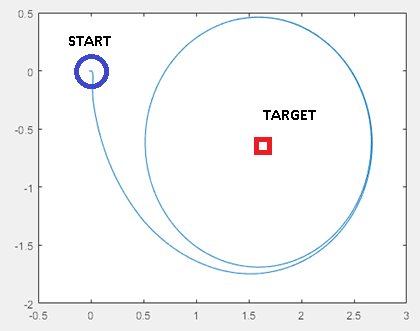
\includegraphics[width=3in]{11}
\caption{Phase Plot of Encirclement Robot} \label{fig:11}
\end{center}
\end{figure}

\begin{figure}[htbp]
\begin{center}
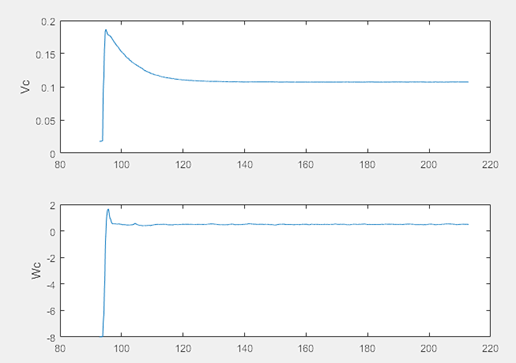
\includegraphics[width=3in]{12}
\caption{Forward and Angular Velocities of Encirclement Robot} \label{fig:12}
\end{center}
\end{figure}

\begin{figure}[htbp]
\begin{center}
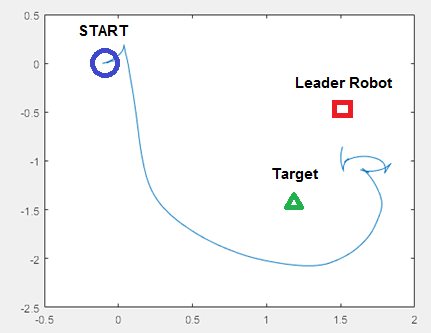
\includegraphics[width=3in]{13}
\caption{Phase Plot of Leader-Follower Robot} \label{fig:13}
\end{center}
\end{figure}

\begin{figure}[htbp]
\begin{center}
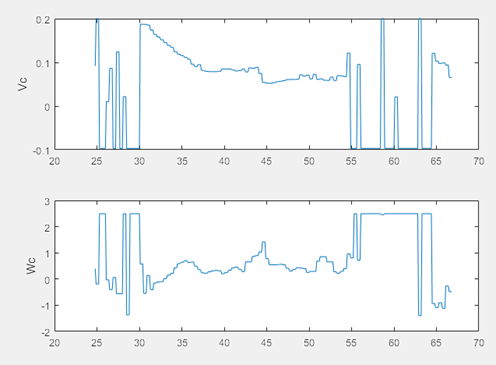
\includegraphics[width=3in]{14}
\caption{Forward and Angular Velocities of Leader-Follower Robot} \label{fig:14}
\end{center}
\end{figure}

\newpage

Video Results:\\
Encirclement control can be seen in the following: \\https://www.youtube.com/watch?v=VHpTNNhiLG4 \\
Leader-follower control can be seen in the following:\\ https://www.youtube.com/watch?v=bO5DHXQCITw




\section{Discussion}

\subsection{Impact of the Design}
Our design allows limited communication and sensing among all robots. Assuming a leader and its peripheral robots, we can obtain encirclement with each consecutive robot containing a smaller and smaller encirclement radii. This two part modular design allows for classifying the leader and followers and allows for increased modularity and customization if needed. With Stateflow, replacing a certain image processing or control module is as simple as replacing or rewriting a Simulink block. Creating simulations for certain environments can also be implemented using Stateflow.
The overall design can be implemented in search and rescue missions, environmental surveying, and much more.

\subsection{Future Work}
There are two areas that can be significantly improved or developed.

The first improvement would be to implement collision avoidance.  This would involve additional image processing as well as control logic.  The kinematic control can be improved to accommodate obstacle avoidance by scaling the encirclement radius as the Qbot2 approaches the obstacle in its path (ref encirclement paper).  As for identifying the obstacle, we believe that this can be accomplished identifying expected distance from the floor and identifying all image elements that deviate from that expected floor distance.  

The method of object recognition could also be improved. One possibility is using edge detection and performing a Hough Transform for the expected target object shape.


% An example of a floating figure using the graphicx package.
% Note that \label must occur AFTER (or within) \caption.
% For figures, \caption should occur after the \includegraphics.
% Note that IEEEtran v1.7 and later has special internal code that
% is designed to preserve the operation of \label within \caption
% even when the captionsoff option is in effect. However, because
% of issues like this, it may be the safest practice to put all your
% \label just after \caption rather than within \caption{}.
%
% Reminder: the "draftcls" or "draftclsnofoot", not "draft", class
% option should be used if it is desired that the figures are to be
% displayed while in draft mode.
%
%\begin{figure}[!t]
%\centering
%\includegraphics[width=2.3in]{myfigure}
% where an .eps filename suffix will be assumed under latex, 
% and a .pdf suffix will be assumed for pdflatex; or what has been declared
% via \DeclareGraphicsExtensions.
%\caption{Simulation results for the network.}
%\label{fig_sim}
%\end{figure}

% Note that the IEEE typically puts floats only at the top, even when this
% results in a large percentage of a column being occupied by floats.


% An example of a double column floating figure using two subfigures.
% (The subfig.sty package must be loaded for this to work.)
% The subfigure \label commands are set within each subfloat command,
% and the \label for the overall figure must come after \caption.
% \hfil is used as a separator to get equal spacing.
% Watch out that the combined width of all the subfigures on a 
% line do not exceed the text width or a line break will occur.
%
%\begin{figure*}[!t]
%\centering
%\subfloat[Case I]{\includegraphics[width=2.3in]{box}%
%\label{fig_first_case}}
%\hfil
%\subfloat[Case II]{\includegraphics[width=2.3in]{box}%
%\label{fig_second_case}}
%\caption{Simulation results for the network.}
%\label{fig_sim}
%\end{figure*}
%
% Note that often IEEE papers with subfigures do not employ subfigure
% captions (using the optional argument to \subfloat[]), but instead will
% reference/describe all of them (a), (b), etc., within the main caption.
% Be aware that for subfig.sty to generate the (a), (b), etc., subfigure
% labels, the optional argument to \subfloat must be present. If a
% subcaption is not desired, just leave its contents blank,
% e.g., \subfloat[].


% An example of a floating table. Note that, for IEEE style tables, the
% \caption command should come BEFORE the table and, given that table
% captions serve much like titles, are usually capitalized except for words
% such as a, an, and, as, at, but, by, for, in, nor, of, on, or, the, to
% and up, which are usually not capitalized unless they are the first or
% last word of the caption. Table text will default to \footnotesize as
% the IEEE normally uses this smaller font for tables.
% The \label must come after \caption as always.
%
%\begin{table}[!t]
%% increase table row spacing, adjust to taste
%\renewcommand{\arraystretch}{1.3}
% if using array.sty, it might be a good idea to tweak the value of
% \extrarowheight as needed to properly center the text within the cells
%\caption{An Example of a Table}
%\label{table_example}
%\centering
%% Some packages, such as MDW tools, offer better commands for making tables
%% than the plain LaTeX2e tabular which is used here.
%\begin{tabular}{|c||c|}
%\hline
%One & Two\\
%\hline
%Three & Four\\
%\hline
%\end{tabular}
%\end{table}


% Note that the IEEE does not put floats in the very first column
% - or typically anywhere on the first page for that matter. Also,
% in-text middle ("here") positioning is typically not used, but it
% is allowed and encouraged for Computer Society conferences (but
% not Computer Society journals). Most IEEE journals/conferences use
% top floats exclusively. 
% Note that, LaTeX2e, unlike IEEE journals/conferences, places
% footnotes above bottom floats. This can be corrected via the
% \fnbelowfloat command of the stfloats package.




\section{Conclusion}
Our project have demonstrated distributed vision-based target tracking control using mobile robots. We have achieved the project goals mentioned in Section 2.3 – that is to design a target identification (detect and locate) module based on RGB image features obtained from a vision sensor, to design a target tracking algorithm based on robot model linearization, to design a leader-follower formation control algorithm based on depth and image features provided from the target identification module, to design a state machine to coordinate target identification module and target control module and communications between robots, and to integrate and validate the proposed distributed controls through experimentation in a controlled lab environment. 
All the while, there were still problems with the upcoming design. The QBot2 does not contain enough processing power for the image processing that we desired – therefore, blob detection was used. A better target recognition algorithm, such as hough transforms, allows a more robust target detection method. Failures, such as the target being misclassified or kinematic issues, were also noted and fixed during implementation. The Qbot occasionally would reset and move backwards once a target object was found. We believe this may be an issue with misclassification or a faulty kinematic model. Another problem with the QBot concerned the updating of RGB and IR images. The middleware for the Simulink design block that increased a tick for every image update occasionally would not change. This prevented us from keeping track each time image processing was finished and delayed search mode.
Overall, this project demonstrated that minimized local communication and formation between robots is feasible. Future work, such as obstacle avoidance and improved image processing, can still be researched.




% conference papers do not normally have an appendix


% use section* for acknowledgment
\section*{Acknowledgment}


Our greatest gratitude goes to Dr. Jing Wang and Dr. In Soo Ahn for their input,
advice, guidance and most of all patience throughout the capstone project. Their
expertise in dynamic systems analysis and understanding of Simulink has helped us
dwelve into the challenging problem of cooperative controls with limited sensing and
communication. Without their help, we would not have gotten as far as we did.
We would also like to thank Mr. Mattus, the ECE Lab Director, for setting up
our development environment and figuring out how to create an ad-hoc network in
Windows 10.
And, we would like to thank Dr. Lu for his assistance in creating this presentation
as well as helping us over the occasional stumbling block in Simulink.
Lastly, we would like to thank our friends and family for their support they have
given us along our journey throughout our college career.





% trigger a \newpage just before the given reference
% number - used to balance the columns on the last page
% adjust value as needed - may need to be readjusted if
% the document is modified later
%\IEEEtriggeratref{8}
% The "triggered" command can be changed if desired:
%\IEEEtriggercmd{\enlargethispage{-3in}}

% references section

% can use a bibliography generated by BibTeX as a .bbl file
% BibTeX documentation can be easily obtained at:
% http://mirror.ctan.org/biblio/bibtex/contrib/doc/
% The IEEEtran BibTeX style support page is at:
% http://www.michaelshell.org/tex/ieeetran/bibtex/
%\bibliographystyle{IEEEtran}
% argument is your BibTeX string definitions and bibliography database(s)
%\bibliography{IEEEabrv,../bib/paper}
%
% <OR> manually copy in the resultant .bbl file
% set second argument of \begin to the number of references
% (used to reserve space for the reference number labels box)
\begin{thebibliography}{1}

\bibitem{}{“Cooperative Control of Heterogenous Mobile Robots Network.” [Online]. Available: http://ee.bradley.edu/projects/proj2016/mrn/. [Accessed:  14-Dec-2016].}

\bibitem{}{G. Bock, R. Hendrickson, J. Lamkin, B. Dhall, J. Wang, and I. S. Ahn, “Experiments of distributed control for multiple mobile robots with limited sensing/communication capacity,” in 2016 IEEE International Conference on Electro Information Technology (EIT), 2016, pp. 0559–0564.}
\bibitem{Oriolo}{G. Oriolo. Wmr control via dynamic feedback linearization: design, implementation and
experimental validation. {\it IEEE Trans. on Control Systems Technology}, 10:835–852, 2002.}
\bibitem{Oriolo}{Franchi, Stegagno, and Oriolo. Decentralized multi-robot encirclement of a 3D target with guaranteed collision avoidance. 2016}
\bibitem{Oriolo}{Freda and Oriolo. Vision-based interception of a moving target with a nonholonomic mobile robot. 2007}
\bibitem{Oriolo}{S. Miah, Lab 2: Trajectory Tracking Using Differential Drive Mobile Robots. 2016 .}
\bibitem{}{Cap 02.pdf. [Online]. \\ Available: http://mayerle.deps.prof.ufsc.br/private/eps6405/Cap 2002.pdf. [Accessed: 14-Nov-2016]}
\bibitem{}{“Kinect for Windows Sensor Components and Specifications.” [Online]. Available: https://msdn.microsoft.com/en-us/library/jj131033.aspx. [Accessed: 14-Dec-2016].}

\bibitem{}{MRNProposalDocument.pdf. [Online]. Available: http://ee.bradley.edu/projects/proj2016/mrn/MRNProposalDocument.pdf.  [Accessed: 14-Nov-2016]}
\bibitem{}P. Corke, Robotics, Vision and Control - Fundamental Algorithms in MATLAB . Sep 2011
\bibitem{}{Quanser - QBot 2 for QUARC. [Online]. Available: http://www.quanser.com/products/qbot2. [Accessed: 14-Nov-2016].}

\end{thebibliography}




% that's all folks
\end{document}


